% Squelette des slides du volet Inférence (5 minutes au total pour le groupe : viser 3-4 slides pour ce volet).
% Compiler depuis ce dossier :  pdflatex inference.tex
% Les figures viennent de :     python plot_results.py --run <run> --reference test --out figures/test
% Notation alignée sur le cours (slides 59-66) : \widehat P (modèle), \widetilde P_a (après rejet), K (budget).
\documentclass[aspectratio=169,11pt]{beamer}
\usetheme{default}
\setbeamertemplate{navigation symbols}{}
\setbeamertemplate{footline}[frame number]
\usepackage[utf8]{inputenc}
\usepackage[T1]{fontenc}
\usepackage[french]{babel}
\usepackage{amsmath,amssymb,booktabs,graphicx}
\graphicspath{{../figures/test/}{../figures/val/}}

\title{Inférence : rejet optimal à budget fixé}
\subtitle{A2 --- GAN MNIST à générateur fixe}
\author{Groupe 3}
\date{}

\begin{document}

% ---------------------------------------------------------------------------------------------------------
\begin{frame}{Question : améliorer l'échantillonnage sans toucher à $G$}
  \begin{columns}[T]
    \column{0.55\textwidth}
    \begin{itemize}
      \item $G$ entraîné et figé, $D$ disponible : peut-on tirer de meilleurs échantillons de $\widehat P$ ?
      \item Baseline : précision $0{,}83$, rappel $0{,}74$, FID $98$ ; chiffre \og 2 \fg{} sous-produit (3,4\,\%), \og 1 \fg{} sur-produit (18,7\,\%).
      \item \textbf{Question} : à budget de calcul $K$ fixé, un rejet piloté par $D$
            augmente-t-il la précision sans perdre de rappel ?
    \end{itemize}
    \column{0.42\textwidth}
    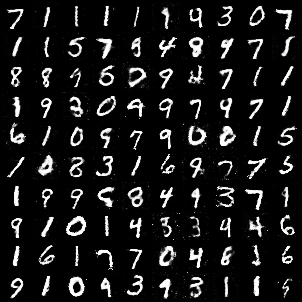
\includegraphics[width=\linewidth]{../figures/samples_checkpoints_plain.png}
  \end{columns}
\end{frame}

% ---------------------------------------------------------------------------------------------------------
\begin{frame}{Méthode : Optimal Budgeted Rejection Sampling (Verine et al., 2024)}
  $D$ optimal $\Rightarrow$ $\dfrac{p(x)}{\widehat p(x)} = \dfrac{D(x)}{1-D(x)} = e^{d(x)}$ \quad ($d$ : logit de $D$)
  \vspace{0.5em}
  \[
    a_{\mathrm{OBRS}}(x) = \min\!\Big(\frac{p(x)}{\widehat p(x)}\frac{c_K}{M},\,1\Big)
                         = \min\!\big(e^{\,d(x)-\tau_K},\,1\big),
    \qquad \mathbb E_{\widehat P}\big[a_{\mathrm{OBRS}}\big] = \tfrac1K
  \]
  \begin{itemize}
    \item Optimal pour toute $f$-divergence à budget $K$ (Thm 3.2) ; $\tau_K$ : bissection sur un pool.
    \item \textbf{Prédiction} (Prop.~3.3) : $(\alpha,\beta) \mapsto (\min\{1, K\alpha\}, \beta)$ :
          précision $\uparrow$, rappel conservé.
    \item Témoins au même coût : DRS (Azadi et al., 2019) ; truncation $z\in[-\psi,\psi]^{100}$ (Brock et al., 2019).
    \item Coût : $K$ passages de $G$ et $D$ par image ; aucun entraînement.
  \end{itemize}
\end{frame}

% ---------------------------------------------------------------------------------------------------------
\begin{frame}{Résultats : précision, rappel et coût}
  \begin{columns}[T]
    \column{0.5\textwidth}
    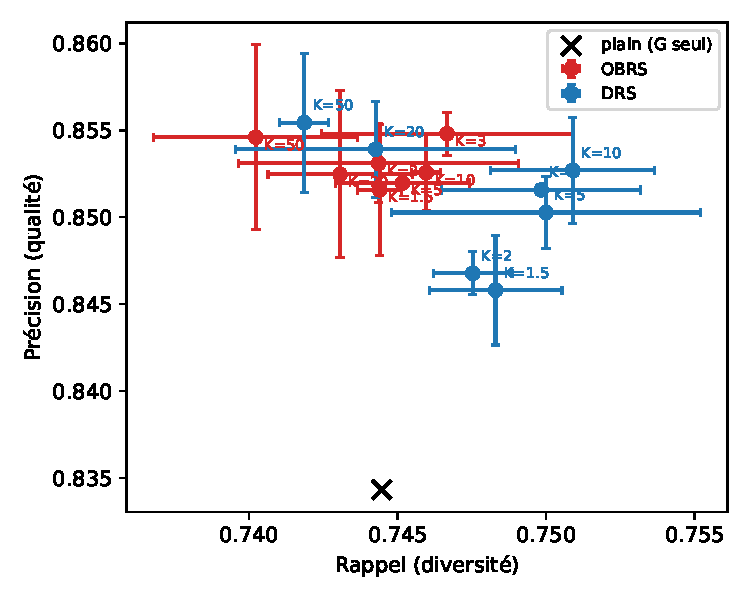
\includegraphics[width=\linewidth]{pr_plane_zoom.pdf}
    \column{0.5\textwidth}
    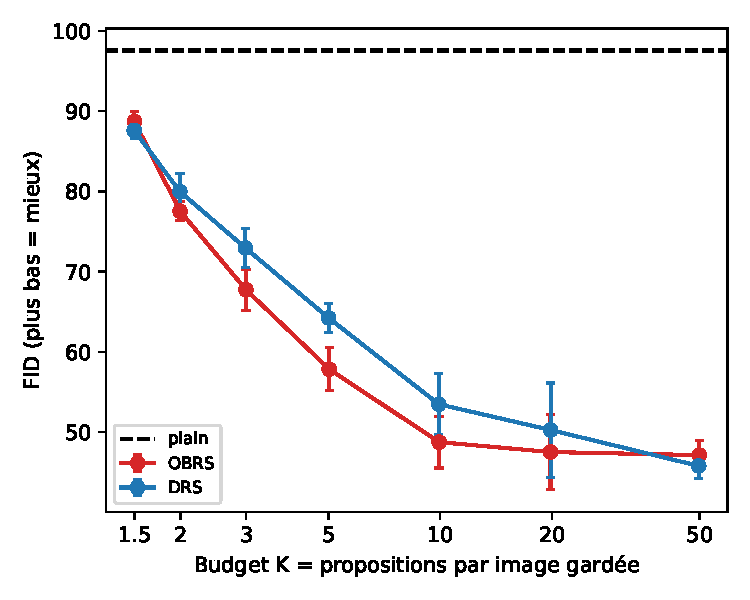
\includegraphics[width=\linewidth]{fid_budget.pdf}
  \end{columns}
  \small 3 seeds, 10\,000 images. OBRS : précision $0{,}834 \to 0{,}853$ à rappel constant ($0{,}744$) ; FID $98 \to 49$ ($K=10$) ; mieux que DRS dans 15/15 paires ($K=2$--$20$).
  % Message : OBRS monte en précision à rappel constant ; DRS en dessous à coût égal ;
  % la truncation gagne en précision mais effondre le rappel.
\end{frame}

% ---------------------------------------------------------------------------------------------------------
\begin{frame}{Analyse : le rejet rééquilibre les classes}
  \begin{columns}[T]
    \column{0.55\textwidth}
    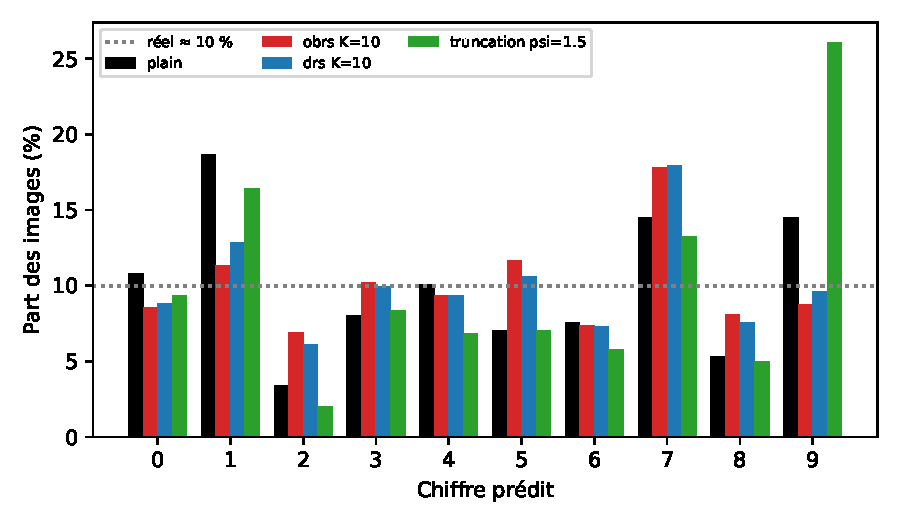
\includegraphics[width=\linewidth]{classes.pdf}
    \column{0.42\textwidth}
    \begin{itemize}
      \item Écart à l'uniforme : $18{,}7\,\% \to 11{,}0\,\%$ ; \og 2 \fg{} : $3{,}4 \to 6{,}9\,\%$.
      \item Truncation : rappel $0{,}74 \to 0{,}35$ ($\psi=1$) : changer $q(z)$ $\neq$ corriger avec $D$.
      \item Limites : $D$ non optimal ; P/R k-NN $\neq$ courbe PRD théorique.
    \end{itemize}
  \end{columns}
\end{frame}

\end{document}
